\documentclass[conf]{new-aiaa}
%\documentclass[journal]{new-aiaa} for journal papers
\usepackage[utf8]{inputenc}

\usepackage{graphicx}
\usepackage{amsmath}
\usepackage[version=4]{mhchem}
\usepackage{siunitx}
\usepackage{longtable,tabularx}
\usepackage[utf8]{inputenc}
\usepackage{amssymb}
\usepackage{graphicx}
\usepackage{hyperref}
\usepackage{subcaption}
\usepackage{sidecap}
\usepackage{mathtools}
% \newcommand{\norm}[1]{\left\lVert#1\right\rVert}
\usepackage{commath}
\usepackage{listings}
\usepackage[version=4]{mhchem}
\usepackage{siunitx}
\usepackage{algorithm}
\usepackage[linewidth=1pt]{mdframed}
\usepackage{algpseudocode}
\usepackage{longtable,tabularx}
\usepackage{amsmath,amsfonts,bm} % Math packages
\usepackage[framed,numbered,autolinebreaks,useliterate]{mcode}
\setlength\LTleft{0pt} 

\title{A 6-DoF Successive Convexification Powered Descent Guidance Implementation using Modified Rodrigues Parameters}

\author{Pádraig S. Lysandrou\footnote{Research Assistant, Aerospace Engineering, AIAA Student Member} and Robert D. Braun\footnote{Smead Professor of Space Technology, Dean of Engineering and Applied Science.}}
\affil{University of Colorado Boulder, Boulder, CO 80309}

\begin{document}

\maketitle

\begin{abstract}
	This paper presents the formulation and demonstration of a 6 degree-of-freedom (DoF) free-final-time guidance algorithm which solves the canonical powered descent guidance (PDG) problem. This formulation can be quickly solved as a series of second order cone program (SOCP) sub-problems making it tractable for online implementation on real-time systems using Interior Point Method (IPM) solvers. Modified Rodrigues Parameters (MRPs), a reduced attitude formalism, are employed in this paper, reducing the number of optimization variables and constraints that other formalisms may bring. It can be initialized with a dynamically inconsistent trajectory and drives the solution to match the nonlinear dynamics with each iteration. This formulation also includes typical vehicular control, environmental, and mission geometry constraint requirements such as thrust vector gimbal angle constraints, glide-slope constraints, and attitude constraints. 

\end{abstract}


\section{Introduction}
\lettrine{T}{he} pin-point landing problem has been of significant interest for a variety of applications. These include safely landing scientific payloads and humans on other planets, returning them back to Earth, and in the reuse of launch vehicles. The capability of reuse of large rocket stages has already proven to be a fundamentally disruptive approach to the launching and has reduced the cost of getting to space \cite{jones2018recent}. Beyond this, landing safely near a base, refueling station, or scientific site will be a necessary technology for the continued exploration of our solar system. It is apparent that robust and reliable powered descent guidance routines will valuable for the future of our space transport infrastructure.

% Optimal control and guidance strategies are generally split into two categories: indirect and direct methods. Although the optimality of the indirect method can be guaranteed, solving the resulted two-point boundary value problem is a difficult task, and good initial guesses of the adjoint variables can be difficult to find or compute. The direct method does not require explicit derivation of first-order necessary conditions; instead, the original optimal control problem is approximated with a parameter optimization problem and solved using nonlinear programming (NLP) algorithms, such as sequential quadratic programming (SQP) algorithms. Although large-scale problems can be handled due to the development of NLP algorithms, the solution process is still time-consuming for complicated problems and dependent upon good initial guesses.

Polynomial Guidance was famously used on the Apollo lunar lander, first landing astronauts on the moon in 1969. The Apollo guidance computer (AGC) had limited compute capability with the algorithms requiring manual re-targeting and flight by the mission pilot. This algorithm was an analytical solution to a boundary valued problem with a fixed time-to-go \cite{klumpp1974apollo}. The final braking law is represented by a quartic polynomial function which connect the initial and terminal states. This result does not satisfy vehicle thrust constraints, and errors introduced by this law must be compensated for by other calculations. Modified versions of this law are still in the literature with an outer time-of-flight search mechanism to effectively make it a free final time-to-go algorithm as well as adding in fuel optimality \cite{d1997optimal}.

More recently, Lossless Convexification was developed to produce a perfect convex second order cone program (SOCP) sub-problem from an originally non-convex problem statement and solve the PDG problem. It is used for convexifying a non-convex constraint without losing any precision, provable via Pontryagin's maximum principle. This method, developed by Açikmeşe, Ploen, and Blackmore is at the heart of the G-FOLD landing algorithm \cite{blackmore2010minimum} \cite{accikmecse2011lossless} \cite{acikmese2012g}. The Guidance algorithm for Fuel Optimal Large Diverts, or G-FOLD, is a recent advancement in PDG solutions. It very quickly calculates a 3DoF fuel optimal divert maneuver with free-final-time, inequality and equality constraints on the states and inputs, and losslessly convexifying the lower thrust constraint. The routine solves a SOCP problem iteratively with an outer time of flight search loop to find the optimal final time. This was successfully demonstrated in a family of flight experiments on Masten Space landing vehicles \cite{acikmese2013flight} \cite{scharf2014adapt}. Similar kinds of problem structures are becoming more popular in aerospace guidance and control \cite{LiuSurvey2017} \cite{wang_paper}. Unfortunately, only a couple types of constraint can be convexified in this fashion, where the remaining nonlinear dynamics are the primary sources of non-convexity.

In this paper, the convex optimization framework is exploited because it is amenable to real-time, on-board implementation and has guaranteed convergence properties with deterministic criteria. These problems can be solved quickly and reliably, especially with custom solvers \cite{dueri2014automated}. The convex programming algorithm to solve powered descent guidance presented herein has non-convex controls constraints and will be posed as a finite-dimensional second-order cone program (SOCP). SOCPs have low complexity and can be solved in polynomial time \cite{nesterov1994interior} \cite{boyd2004convex}.

A method called successive convexification or SCvx, championed by \cite{mao2016successive}, is employed and this paper is largely based on the work of Szmuk et al \cite{szmuk2018successive}. In this method, the algorithm is initialized with a reference trajectory, then linearized and discretized as an SOCP problem. The problem is then structured as an iterative solution process where the current problem is linearized about the previous trajectory. This is done in such a way that the solution satisfies the original nonlinear dynamics, non-convex constraints, and other state and control constraints. On each iteration, the dynamic relaxation weights are tightened to adhere closer to the true dynamics.

The goal of the presented algorithm is to generate optimal translational and attitude trajectory profiles that are dynamically feasible. This means that the modeled vehicle should abide by all state boundary conditions, actuator constraints, and the proposed dynamics. This problem will first be defined as a continuous-time non-convex dynamical problem and then converted to a disciplined convex program. The dynamic, control, initial, and terminal constraints that must be met throughout the problem will also be discussed and derived. In order to maximize the divert capability of the vehicle, an objective of minimizing the final time of the solution is proposed. Although not proven here, this can be considered a proxy to the minimum-fuel consumption problem, as the non-convex constraint of minimum-thrust and single-ignition requires that the engine be on for the duration of the landing phase. In this scenario, the fuel-consumption cost is strictly increasing monotonic, and the sooner the terminal conditions can be met, the fewer the total cost. A similar free-ignition-time modification can be made to further decrease this cost and  optimize the ignition time \cite{szmuk2019successive}. 

\subsection{On Successive Convexification}
The successive convexification framework (SCvx) is able to quickly solve optimal control problems with nonlinear dynamics and non-convex state and control constraints \cite{szmuk2018successive}. It does this by iteratively solving convex optimization sub-problems, obtained by linearizing non-convexities in dynamics and constraints around the previous iteration solution. These sub-problems employ techniques of virtual control (dynamic relaxation), virtual buffer zones, and trust regions to prevent solution artificial infeasibility and artificial unboundedness. This linearization acts as an approximation, but the solution is driven to convergence within the user's tolerances to solve exactly the originally proposed non-convex optimal control problem with local optimality.

Methods like sequential convex programming (SCP) offers a way to solve problems with more general nonlinear dynamics and non-convex constraints. While SCP performs well empirically, no general convergence results have been reported. SCvx differs from other SCP approaches in many ways, including proofs for (weak and strong) global convergence and superlinear convergence rate \cite{mao2016successive}. For general real-time autonomy tasks where safety and determinism are prioritized, it is often much better to find a locally optimal solution quickly rather than a globally optimal solution slowly. Generally speaking, nonlinear programming tends to be the method of choice for locally optimal solutions. However, their convergence behaviour is dependent upon the initial guess provided to the solver and do not offer bounds on computational effort required for convergence. These facts are at odds with requirements for real-time embedded applications.

\subsection{Definitions and Notation}
The $\mathcal{F}_\mathcal{N} : \{\mathcal{O}_\mathcal{N}, \hat{\bm{n}}_1, \hat{\bm{n}}_2, \hat{\bm{n}}_3 \}$ frame defines an inertially fixed Up-East-North reference frame where the origin $\mathcal{O}_\mathcal{N}$ located at the landing site. This can easily be changed to the local-vertical local-horizontal (LVLH) or other useful frame definition. The $\mathcal{F}_\mathcal{B}: \{\mathcal{O}_\mathcal{B}, \hat{\bm{b}}_1, \hat{\bm{b}}_2, \hat{\bm{b}}_3 \}$ frame is a body fixed frame where the x-axis is aligned vertically with the vehicle, or aligned with the thrust vector at zero thrust vector control (TVC) deflection angle. The Y-axis points out of the side of the cylindrical vehicle and the Z-axis completes the right handed triad.

Here forward, it should also be assumed that the vectorial derivative, shown by $\mathbf{\dot{r}}$, is an inertial time derivative. Derivatives in frames other than the inertial frame will be indicated otherwise as $^\mathcal{X}\frac{d \mathbf{r}}{dt}$. Any vector shown as $^\mathcal{X}\mathbf{r}$ is in the $\mathcal{X}$ frame, and similarly anything without this left superscript is frameless. Therefore the vector $\bm{\omega}_{\mathcal{B/N}}$ is the frameless angular velocity vector of the body frame with respect to the inertial frame. The notation $\mathbb{R}$, $\mathbb{R}_+$, and $\mathbb{R}_{++}$ is used to denote the set of real values, non-negative real values, and positive real values respectively.


\section{Vehicle Dynamics}
\subsection{Translational Dynamics}
Given that most powered descent maneuvers are done within kilometers of a site, and at speeds much less than orbital velocities, a simplified gravitational acceleration assumption with a non-rotation planet is used. Similarly, aerodynamic forces are assumed to be negligible, representative of a Mars or lunar landing scenario. However, as shown in a later section, any nonlinear dynamics can be incorporated, as they will be represented as a linear time-varying (LTV) system which is successively convexified to solve the nonlinear problem exactly to a locally optimum solution. Therefore, the linearization and discretization scheme employed allow for additional nonlinear terms. 

The algorithm as presented has the vehicle actuated by a single gimbaled thruster at the bottom of the vehicle. It should be stated that the algorithm can readily accommodate other actuators, actuator geometries, and configurations. This engine has feasible thrust magnitude and efficiency, as well as standard gimbal range for agile landing or vertical-takeoff-vertical-landing (VTVL) vehicles. To be inclusive of actuator dynamics, it is assumed that the engine has maximum and minimum thrust bounds. Most rocket engines have a minimum throttle percentage, below which the engine does not perform well or in a stable manner. Similarly, during the powered descent regime, a single ignition occurs; the engine is not turned off or re-ignited until commanded at the terminal state. This minimum thrust constraint is a source of non-convexity \cite{accikmecse2011lossless}.

It is critical to capture the mass depletion dynamics, proportional to the magnitude of the thrust generated by the engine. For simplicity, the inertia matrix and the position of the center-of-mass is assumed to be constant throughout the trajectory although these modifications can also be included in the dynamic formulation. The constant $\alpha_{\dot{m}}$, a function of the specific impulse, is used as the mass depletion parameter. This is the inverse of the mass flow rate, which is the total flow rate of the propellants to the engine. Additionally, a constant specific impulse throughout the throttleable region is assumed, which may not always be true. Normally, an engine operating at a lower thrust than nominal may may be less efficient and have a lower specific impulse. These effects are small enough to be ignored in this problem statement. Therefore,
% 
\begin{align}
& \alpha_{\dot{m}} = \frac{1}{I_{sp} g_0} \\
& \dot{m}(t) = -\alpha_{\dot{m}} \left\lVert \mathbf{F}_{thrust}(t) \right\rVert _2
\end{align}
% 
With the assumptions made, the translational dynamics and forces acting on the vehicle in the inertial frame can be derived. They are as follows:
% 
\begin{align}
& \dot{\mathbf{r}}(t) = \mathbf{v}(t) \\
& \dot{\mathbf{v}}(t) = \frac{\mathbf{F}_{thrust}(t)}{m(t)} + \mathbf{g}
\end{align}
where $\mathbf{g}$ is the static, spherical planetary gravitation vector. As stated previously, any extra nonlinear terms can be added to this formulation and they will be solved exactly. This may become useful in the hypersonic entry, supersonic retropropulsive, or any perturbing regimes. Moving forward, the translational dynamics are assumed to be in the inertial frame and all rotational dynamics to be in the body fixed frame.

\subsection{Attitude Dynamics and Formalism}
In this formulation, the vehicle is treated as a rigid body. From Euler's principal rotation theorem,  any coordinate reference frame can be brought from an arbitrary initial condition to an arbitrary final orientation by a single rigid rotation through a principle angle $\phi$ about a principal axis $\hat{\bm{e}}$. This axis is fixed in both the initial and final orientation. Therefore $\hat{\bm{e}} = [C]\hat{\bm{e}}$, where $[C]\in SO(3)$ is a rotation mapping in $\mathbb{R}^{3\times3}$ taking a vector from the initial orientation to the final, shows that $\hat{\bm{e}}$ is an unit eigenvector of the $[C]$ transform whose eigenvalue is $+1$. This rotation mapping matrix, a direction cosine matrix (DCM), has nine parameters and can be cumbersome although exact. For ease of manipulation, it is preferred to use mappings with fewer parameters.

\subsubsection{Modified Rodrigues Parameters}
Another minimal attitude formalism are the Modified Rodrigues Parameters (MRPs). 
MRPs are a popular mechanism which forms a three parameter set without a norm constraint. They are derived from quaternions, as shown in \ref{mrp}
%
\begin{align}
\label{mrp}
	\sigma_i &= \frac{q_i}{1+q_0} \quad i = 1,2,3 \\
	\boldsymbol{\sigma}_\mathcal{B/N} &= [\sigma_1 \ \sigma_2 \ \sigma_3]^T = \tan\frac{\phi}{4}\hat{\bm{e}}
\end{align}
taking a scalar-first quaternion argument of $\bm{q}_\mathcal{B/N}$. The reverse mapping is simply $q_0 = \frac{1-\sigma^2}{1+\sigma^2}$ and $q_{1:3} = \frac{2\sigma_{1:3}}{1+\sigma^2}$ where $\sigma^2$ here forward will represent the norm squared of the MRP. With MRPs, small angle approximations can be made for a wider range of displacements. It is clear that there exists a singularity at $\pm 2\pi$. However, handling this singularity, in a computational sense, is very simple. A switch can be performed to the MRP shadow set when the angular displacement is $\phi \geq \pi$ and define the shadow set as $\boldsymbol{\sigma}^\mathcal{S} = \frac{-\boldsymbol{\sigma}}{\sigma^2} = \tan{\frac{\phi-2\pi}{4}}\hat{\bm{e}}$. 

If we constrain the dynamics such that a vehicle does not undergo a full rotation, we can simply constrain the MRP once and minimize problem complexity. In optimization routines where large angular displacements must be made, it could be possible to encode state triggered switching events to produce this behavior \cite{szmuk2019successive}. It should be recognized that the MRP-to-DCM mapping will be required:
\begin{align}
\label{mrp2c}
	C_{\mathcal{B/N}} = [\mathcal{BN}]= \mathbb{I}_3 +  \frac{8[\boldsymbol{\sigma}^\times]^2 - 4(1-\sigma^2)[\boldsymbol{\sigma}^\times]}{(1+\sigma^2)^2}
\end{align}
taking an argument of $\boldsymbol{\sigma}_\mathcal{B/N}$ and where $\mathbb{I}_3$ is the identity matrix. The kinematic differential equation is \ref{mrpkde}
%
\begin{align}
\label{mrpkde}
	\dot{\boldsymbol{\sigma}} = \frac{1}{4}[(1-\sigma^2)\mathbb{I}_3 +  2[\boldsymbol{\sigma}^\times] + 2\boldsymbol{\sigma}\boldsymbol{\sigma}^T] \ ^\mathcal{B}\boldsymbol{\omega}_\mathcal{B/N} = \frac{1}{4}B_\sigma(\boldsymbol{\sigma}) \ ^\mathcal{B}\boldsymbol{\omega}_\mathcal{B/N}
\end{align}
as a function of the body frame vehicle angular rate.

Differentiating the angular momentum vector of system, and making the rigid body assumption, an equation of motion emerges:
\begin{align}
\dot{\bm{H}} &= \mathbf{L}_c = [I_c]\dot{\boldsymbol{\omega}} + [\boldsymbol{\omega}^\times][I_c]\boldsymbol{\omega}
\end{align}
where the torque acting on the vehicle is written as $\mathbf{L}_c(t) \in \mathbb{R}^3$ in the body frame. Rearranged, the canonical Euler rotational equations of motion appears:
\begin{align}
	\dot{\boldsymbol{\omega}} = [I_c]^{-1}(\mathbf{L}_c - [\boldsymbol{\omega}^\times][I_c]\boldsymbol{\omega})
\end{align}
While the moment of inertia matrix would normally be determined from the design of the vehicle, a cylinder rotating about it's center with a homogeneous mass distribution is assumed for this presentation.


\section{Boundary Conditions and State Constraints}
The boundary conditions for the proposed guidance routine are simple. The state vector initial and desired terminal condition of the vehicle must both be hard boundary constraints. The initial boundary constraint is set at the initialization of the routine. Therefore, they are:
\begin{align}
	m(0) = m_0, \quad ^\mathcal{N}\mathbf{r}(0) = \mathbf{r}_0, \quad ^\mathcal{N}\mathbf{v}(0) = \mathbf{v}_0, \quad \boldsymbol{\sigma}_\mathcal{B/N}(0) = \boldsymbol{\sigma}_0, \quad  ^\mathcal{B}\boldsymbol{\omega}_\mathcal{B/N}(0) = \boldsymbol{\omega}_0
\end{align}
Similarly, the terminal state boundary constraint is the following:
\begin{align}
	\quad ^\mathcal{N}\mathbf{r}(0) = \mathbf{0}, \quad ^\mathcal{N}\mathbf{v}(0) = \mathbf{0}, \quad \boldsymbol{\sigma}_\mathcal{B/N}(0) = \mathbf{0}, \quad  ^\mathcal{B}\boldsymbol{\omega}_\mathcal{B/N}(0) = \mathbf{0}
\end{align}
leaving the final mass unconstrained and assuming the landing site to be the origin. An upright attitude is also assumed, given that the vehicle has landing hardware in this orientation. Of course these can be modified to fit arbitrary landing requirements. The problem proposed in \cite{szmuk2018successive} does not constrain the initial attitude of the vehicle, but it is constrained in this formulation. It may not be a bad assumption as the attitude control bandwidth is normally larger than the translational control bandwidth in addition to minimizing the number of system constraints.

Now, let us look at the state constraints that must be met. The vehicle propulsion system is limited in fuel which manifests itself as this inequality constraint:
\begin{align}
& m_{dry} - m(t) \leq 0
\end{align}
%
Let us apply a glide-slope constraint such that the vehicle approaches the landing point from above, limiting large lateral diverts in the terminal phase. A convex constraint  is formed using the angle $\gamma_{gs}$. This becomes a simple geometrical argument that $\tan{\gamma_{gs}} \leq \frac{r_{Up}}{\norm{[ r_{East} \ r_{North}]}}$. This is formed with the following:
\begin{align}
\tan{\gamma_{gs}} || [\hat{\bm{n}}_2 \quad \hat{\bm{n}}_3 ]^T \mathbf{r}(t) \lvert\lvert_2 \ - \ \hat{\bm{n}}_1^T \mathbf{r}(t) \leq 0
\end{align}
This  creates an upward facing cone about the landing point that the vehicle must not lie outside of. This type of convex constraint can also be useful in avoiding rocky terrain and enforcing a landing from directly above a target, minimizing lateral movement close to the ground. Additionally, one could implement super-terminal velocity constraints which constrain the lateral movement to zero as the vehicle approaches the landing position.


It is also helpful to restrict the attitude of the vehicle such that it does not tilt over a prescribed angular displacement. This could be to maintain visibility for terrain relative navigation sensors or to give human passengers visibility over the terrain or landing surface. Therefore the angle between the inertial frame ``up'' unit vector and the bore-sight body vector of the vehicle can be constrained. The constraint derivation begins with $\hat{\bm{b}}_1 \cdot \hat{\bm{n}}_1 \geq \cos{\psi_{max}}$:
\begin{align}
	\left (
	[\mathcal{NB}]
	\prescript{\mathcal{B}}{}{
	\begin{bmatrix}
		1 \\ 0 \\ 0
	\end{bmatrix}}
	\right )^T \
	\prescript{\mathcal{N}}{}{
	\begin{bmatrix}
		1 \\  0 \\ 0
	\end{bmatrix}}
	\geq \cos{\psi_{max}}
\end{align}
this selects the $(1,1)$ element of the MRP-to-DCM matrix in equation \ref{mrp2c}. Therefore the constraint becomes:
%
\begin{align}
\label{alignconstraint}
	1- \frac{8(\sigma_2^2 + \sigma_3^2)}{(1+\sigma^2)^2} \geq \cos{\psi_{max}}
\end{align}
This quaternion version of this same constraint is $1-2(q_{2}^{2}+q_{3}^{2}) \geq \cos(\psi_{max})$. The quaternion unity identity must be used in this derivation. The quaternion definition is convex, but the MRP version is not. However, this issue can be circumnavigated by using the direct MRP identity $\boldsymbol{\sigma}_\mathcal{B/N} = \tan\frac{\phi}{4}\hat{\bm{e}}$. Therefore, the entire MRP can be constrained such that the vehicle does not exceed $\psi_{max}$ radians in total angular displacement from the zero angle, which will suffice for our application. The zero MRP is defined as the upward unit vector in the target inertial frame.
\begin{align}
	\left \lVert \boldsymbol{\sigma}_\mathcal{B/N} (t) \right \lVert_2 \leq \tan \left( \frac{\psi_{max}}{4} \right)
\end{align}
Most divert maneuvers should have relatively small angular rates, and can be bounded for descent and landing. This can simply be constrained as well.
\begin{align}
& \left \lVert \bm{\omega}_\mathcal{B/N}(t) \right \lVert_2 \leq \omega_{max}
\end{align}

Finally the commanded thrust magnitude must be constrained. As stated before, engines have a minimum and maximum thrust region $[T_{min}, T_{max}] \in \mathbb{R}_{++}$ in which they operate. Additionally, recall the single-ignition assumption. Finally, the engine thrust vector control system has a dynamic range with limited angular deflection $\delta_{\text{TVC}_{max}}$.
\begin{align}
& 0 < F_{min} \leq \left \lVert \bm{F}_{thrust}(t) \right \lVert_2 \leq F_{max} \\
& \cos(\delta_{\text{TVC}_{max}}) \left \lVert \bm{F}_{thrust}(t) \right \lVert_2 \leq \hat{\bm{b}}_1^T \bm{F}_{thrust}(t)
\end{align}
It is clear that the upper thrust bound is convex. However, the lower bound creates a non-convex constraint \cite{accikmecse2011lossless}. Other formulations show this can be losslessly convexified, but in the problem implemented herein, the nonconvexity will be handled via linearization in the discretization step discussed in a later section.

%
\section{Continuous Time Problem Statement}

Putting this all together, let us pose the continuous time optimization problem. In this form, it is non-convex and requires conditioning to work into the convex programming framework. As stated, the objective is to minimize the time-of-flight required to get to the terminal conditions subject to the aforementioned constraints, dynamics, and boundary conditions. The state vector, thrust commands, gimbal angles, and final time are optimization variables and are considered the solution to this problem. This is posed in Problem one: \ref{ctproblem}.


\clearpage
\begin{mdframed}
\label{ctproblem}
\textbf{Problem 1: Continuous Time Non-Convex Free-Final-Time}
\newline
\underline{Cost Function:}
\begin{equation*}
\min_{\mathbf{x}, \ \mathbf{F}_{th}} t_f
\end{equation*}
%
\underline{Boundary Conditions:}  
\begin{align*}
m(0) &= m_0, &^\mathcal{N}\mathbf{r}(0) &= \mathbf{r}_0, & ^\mathcal{N}\mathbf{v}(0) &= \mathbf{v}_0, & \boldsymbol{\sigma}_\mathcal{B/N}(0) &= \boldsymbol{\sigma}_0, \quad ^\mathcal{B}\boldsymbol{\omega}_\mathcal{B/N}(0) = \boldsymbol{\omega}_0 \\
\quad ^\mathcal{N}\mathbf{r}_{T} &= \mathbf{0}, & ^\mathcal{N}\mathbf{v}_T &= \mathbf{0}, & \boldsymbol{\sigma}_{\mathcal{B/N}_T} &= \mathbf{0}, & ^\mathcal{B}\boldsymbol{\omega}_{\mathcal{B/N}_{T}} &= \mathbf{0}
\end{align*}
%
\underline{Dynamics:}  
\begin{align*}
\dot{m}(t) &= -\alpha_{\dot{m}} \left\lVert \mathbf{F}_{th}(t) \right\rVert _2 \\
^\mathcal{N}\dot{\mathbf{r}}(t) &= \mathbf{v}(t) \\
^\mathcal{N}\dot{\mathbf{v}}(t) &= \frac{[\mathcal{NB}(\boldsymbol{\sigma})] \ ^\mathcal{B}\mathbf{F}_{th}(t)}{m(t)} +  \ ^\mathcal{N}\mathbf{g} \\
\dot{\boldsymbol{\sigma}}_\mathcal{B/N} &= \frac{1}{4} \left [(1-\sigma^2)\mathbb{I}_3 +  2[\boldsymbol{\sigma}^\times] + 2\boldsymbol{\sigma}\boldsymbol{\sigma}^T \right ] \ ^\mathcal{B}\boldsymbol{\omega}_\mathcal{B/N} \\
^\mathcal{B}\dot{\boldsymbol{\omega}}_\mathcal{B/N} &= [I_c]^{-1}\left([\boldsymbol{r}_{\text{COM}}^\times] \ ^\mathcal{B}\mathbf{F}_{th}(t) - [\boldsymbol{\omega}^\times][I_c]\boldsymbol{\omega}\right)
\end{align*}
%
\underline{State and Control Constraints:}  
\begin{align*}
m_{dry} - m(t) & \leq 0 \\
|| [\hat{\bm{n}}_2 \ \ \hat{\bm{n}}_3 ]^T \mathbf{r}(t) \lvert\lvert_2 \ \tan{\gamma_{gs}}  - \hat{\bm{n}}_1^T \mathbf{r}(t) & \leq 0 \\
%
\left \lVert \boldsymbol{\sigma}_\mathcal{B/N} (t) \right \lVert_2 &\leq \tan \left( \frac{\psi_{max}}{4} \right) \\
%
\left \lVert \bm{\omega}_\mathcal{B/N}(t) \right \lVert_2 & \leq \omega_{max}\\
0 < F_{min} \leq \left \lVert \bm{F}_{th}(t) \right \lVert_2 &\leq F_{max} \\
\cos(\delta_{max}) \left \lVert \bm{F}_{th}(t) \right \lVert_2 &\leq \hat{\bm{b}}_1^T \bm{F}_{th}(t)
\end{align*}
\end{mdframed}




% ####################################################################################
% ####################################################################################
% ####################################################################################

\section{Linearization}
Now the convex form of Problem 1 shall be derived. The non-convex continuous free-final-time problem is converted into a convex fixed-final-time problem. This will be a second order cone sub-problem. This sub-problem is solved repeatedly to convergence or ``successively.'' This successive process turns each subproblem into a larger free-final-time algorithm.
Let us define the state vector $\mathbf{x}(t) \in \mathbb{R}^{13\times 1}$ and our control vector $\mathbf{u}(t) \in \mathbb{R}^{3\times 1}$:
\begin{align}
& \mathbf{x}(t) \triangleq 
	\begin{bmatrix}
	m(t) & ^\mathcal{N}\mathbf{r}^T(t) & ^\mathcal{N}\mathbf{v}^T(t) & \boldsymbol{\sigma}_\mathcal{B/N}^T(t) & ^\mathcal{B}\bm{\omega}_\mathcal{B/N}^T(t)   
	\end{bmatrix}^T \\
& \mathbf{u}(t) \triangleq \ ^\mathcal{B}\mathbf{F}_{th}(t)  
\end{align}
Therefore the nonlinear dynamics can be expressed in the following form:
\begin{align}
& \frac{d}{dt}\mathbf{x}(t) = \mathbf{f}(\mathbf{x}(t), \mathbf{u}(t)) =  
	\begin{bmatrix}
	\dot{m}(t) & ^\mathcal{N}\dot{\mathbf{r}}^T(t) & ^\mathcal{N}\dot{\mathbf{v}}^T(t) & \dot{\boldsymbol{\sigma}}_\mathcal{B/N}^T(t) & ^\mathcal{B}\dot{\bm{\omega}}_\mathcal{B/N}^T(t)  
	\end{bmatrix}^T
\end{align}

In order to formulate our guidance problem with a free-final-time objective, time dilation is introduced. Let us evaluate our dynamics on a normalized trajectory time variable $\tau \in [0,1]$. No matter the resolution of the optimization, the terminal value will end at $\tau = 1$. A differentiation based on this variable is then used to scale the time back and forth, leaving the unscaled final time as an optimization variable. Applying the chain rule of differentiation: 
\begin{align}
& \mathbf{f}(\mathbf{x}(t) , \mathbf{u}(t)) =  \frac{d}{dt}\mathbf{x}(t) = \frac{d\tau}{dt} \frac{d}{d\tau}\mathbf{x}(t) =  \frac{1}{\eta}\frac{d}{d\tau}\mathbf{x}(t)
\end{align}
Let us now translate between the two by using the dilation coefficient $\eta$ which is define as
\begin{align}
& \eta \triangleq \left(\frac{d\tau}{dt}\right)^{-1}
\end{align}

This $\eta$ will become a variable in the convex subproblem that acts as the non-dimensionalized final time. It is a scaling factor that translates between real work differential time and the normalized version used for our algorithm. The nonlinear dynamics, taking advantage of this normalized time, are then written as:
\begin{align}
& \mathbf{x}^\prime(\tau) \triangleq \frac{d}{d\tau}\mathbf{x}(\tau) = \eta \  \mathbf{f}(\mathbf{x}(\tau), \mathbf{u}(\tau)) = \mathbf{g}(\mathbf{x}(\tau), \mathbf{u}(\tau), \eta)
\end{align}

Taking a first-order Taylor series approximation of the nonlinear dynamics proposed in problem one (\ref{ctproblem}), a linear time-varying system of equations is written to use in our algorithm shown in \ref{taylor}. These dynamics will be instantiated at reference values $(\hat{\mathbf{x}}, \hat{\mathbf{u}}, \hat{\eta})$ at each time, together being referred to as the \textit{linearization path}. 
%
\begin{subequations}
\label{taylor}
\begin{align}
\mathbf{x}^\prime(\tau) 
&= \mathbf{g}(\hat{\mathbf{x}}(\tau), \hat{\mathbf{u}}(\tau), \hat{\eta})
+ \frac{\partial \mathbf{g}}{\partial \mathbf{x}} \bigg\rvert_{\hat{x},\hat{u},\hat{\eta}} (\mathbf{x} - \hat{\mathbf{x}}) \ 
+ \frac{\partial \mathbf{g}}{\partial \mathbf{u}} \bigg\rvert_{\hat{x},\hat{u},\hat{\eta}} (\mathbf{u} - \hat{\mathbf{u}}) \ 
+ \frac{\partial \mathbf{g}}{\partial \eta} \bigg\rvert_{\hat{x},\hat{u},\hat{\eta}} (\eta - \hat{\eta}) \\
&= \hat{\eta} \mathbf{f}(\hat{\mathbf{x}}(\tau), \hat{\mathbf{u}}(\tau))
+ \hat{\eta} \frac{\partial \mathbf{f}}{\partial \mathbf{x}} \bigg\rvert_{\hat{x},\hat{u}} (\mathbf{x} - \hat{\mathbf{x}}) \
+ \hat{\eta} \frac{\partial \mathbf{f}}{\partial \mathbf{u}} \bigg\rvert_{\hat{x},\hat{u}} (\mathbf{u} - \hat{\mathbf{u}}) \
+ \mathbf{f}(\hat{\mathbf{x}}(\tau), \hat{\mathbf{u}}(\tau)) (\eta - \hat{\eta}) \\
&= {\eta} \mathbf{f}(\hat{\mathbf{x}}(\tau), \hat{\mathbf{u}}(\tau))
+ \hat{\eta} \frac{\partial \mathbf{f}}{\partial \mathbf{x}} \bigg\rvert_{\hat{x},\hat{u}} (\mathbf{x} - \hat{\mathbf{x}}) \
+ \hat{\eta} \frac{\partial \mathbf{f}}{\partial \mathbf{u}} \bigg\rvert_{\hat{x},\hat{u}} (\mathbf{u} - \hat{\mathbf{u}}) \\ 
& = \Sigma(\tau)\eta + A(\tau) (\mathbf{x} - \hat{\mathbf{x}}) + B(\tau)(\mathbf{u} - \hat{\mathbf{u}})  \\ 
&= \Sigma(\tau)\eta + A(\tau)\mathbf{x} + B(\tau)\mathbf{u} + \mathbf{z}(\tau)
\end{align}
\end{subequations}

This expression is simplified by breaking the Taylor expansion intro matrix subcomponents. 
\begin{align}
& A(\tau) \triangleq \hat{\eta} \frac{\partial \mathbf{f}}{\partial \mathbf{x}}  \bigg\rvert_{\mathbf{\hat{x}}, \mathbf{\hat{u}}} \\
& B(\tau) \triangleq \hat{\eta} \frac{\partial \mathbf{f}}{\partial \mathbf{u}}  \bigg\rvert_{\mathbf{\hat{x}}, \mathbf{\hat{u}}} \\
& \Sigma(\tau) \triangleq \mathbf{f}(\hat{\mathbf{x}}(\tau), \hat{\mathbf{u}}(\tau)) \\
& \mathbf{z}(\tau) \triangleq -A(\tau)\mathbf{\hat{x}}- B(\tau)\mathbf{\hat{u}}
\end{align}





\addtocontents{toc}{\protect\setcounter{tocdepth}{1}}
\subsection{Convexifying the Minimum Thrust Constraint}
\addtocontents{toc}{\protect\setcounter{tocdepth}{2}}
Let us now tackle the last source of non-convexity: the non-zero lower bound on actuator thrust. Let us define an $\mathbb{R}^3 \rightarrow \mathbb{R}$ mapping function: $g(\mathbf{u}(\tau)) = F_{min} - \norm{\mathbf{u}(\tau)}_2 \leq 0$. Taking the first order Taylor series linear approximation, the following convexified constraint formulation becomes:
%
\begin{align}
	g(\mathbf{u}(\tau)) &= F_{min} - \norm{\hat{\mathbf{u}}(\tau)} - \frac{\hat{\mathbf{u}}(\tau)^T}{\norm{\hat{\mathbf{u}}(\tau)}}(\mathbf{u}(\tau) - \hat{\mathbf{u}}(\tau)) & \leq 0 \\
	&= F_{min} - \frac{\hat{\mathbf{u}}(\tau)^T}{\norm{\hat{\mathbf{u}}(\tau)}} \mathbf{u}(\tau)  & \leq 0\\
	&= F_{min} - \Xi(\tau)\mathbf{u}(\tau)  & \leq 0
\end{align}
this leads us to the linear, convexified constraint $F_{min} \leq \Xi(\tau)\mathbf{u}(\tau)$ requiring the linearization path value $\hat{\mathbf{u}}(\tau)$. This means that each iteration of the algorithm will use the input sequence path from the previous iteration to satisfy this constraint.







\section{Discretization Scheme}
The final step to fitting the dynamics, state, and control constraints to an optimization form is to cast the problem as a finite dimensional discretization. This finite dimensional problem is chosen to occur over $K\in\mathbb{Z}$ evenly separated points with respect to the normalized trajectory time $\tau$. The index set is defined as $\mathcal{K}\in\mathbb{Z}^{K}$ and $\mathcal{K}_-\in\mathbb{Z}^{K-1}$ for the state and input histories as the following:
\begin{align*}
	\mathcal{K} &\triangleq \{0,1,\cdots, K-1\} \\
	\mathcal{K}_- &\triangleq \{0,1,\cdots, K-2 \}
\end{align*}
%
Given that the trajectory time is normalized on the interval $\tau \in [0,1 ]$, the discrete time step at point $k$ is defined as such:
%
\begin{align}
& \tau_k \triangleq \frac{k}{K-1}, \quad \forall k \in \mathcal{K}
\end{align}
%
For the sake of implementation, a first-order-hold linear scaling is applied to the controls for each time step. Over the interval $\tau \in [\tau_k, \tau_{k+1}]$, the $\mathbf{u}(\tau)$ is expressed in terms of the $\mathbf{u}_k$
 and $\mathbf{u}_{k+1}$:
\begin{equation}
	\mathbf{u}(\tau) \triangleq \alpha_k(\tau) \mathbf{u}_k + \beta(\tau) \mathbf{u}_{k+1}
\end{equation}
%
The input is spread linearly, on a first order relationship, from the index position $k$ to the next known control value at $k+1$ in the control history. This also allows us to consider controller interpolation scheme a priori if used in a feed forward regime. The successive convexification algorithm was tested with a number of discretization methods on state and input, where first order hold (FOH) and Legendre-Gauss-Radau (LGR) collocation methods were found to be the most amenable \cite{malyuta2019discrete}. These two provided the fastest computation times with good performance.
%
The previously defined constants follow the following form:
\begin{align}
d\tau &= \frac{1}{K-1} \\
\alpha_k(\tau) &= \frac{d\tau - \tau}{d\tau} \\
\beta_k(\tau) &= \frac{\tau}{d\tau}
\end{align}
%

The state transition matrix (STM) of the dynamics $\Phi(\tau_{k+1},\tau_k)$ is used to translate the process from a state at time $k$ to future state at $k+1$. This matrix assumes no input is being imparted, but a convolution can be used to describe the time varying input. The STM follows the dynamics:
%
\begin{align}
& \frac{d}{d\tau} \Phi(\tau,\tau_k) = A(\tau) \Phi(\tau,\tau_k), \quad \forall k \in \mathcal{K}
\end{align}
Additionally, the STM has the semigroup, inverse, and identity properties which become useful in the derivation:
\begin{align}
	\Phi(t,s) &= \Phi(t, \gamma)\Phi(\gamma, s) \\
	\Phi(t,s)^{-1} &= \Phi(s,t) \\
	\Phi(s,s) &= \mathbb{I}_{n \times n}
\end{align}
for arbitrary timing parameters $t, \gamma, s$. Let us take advantage of this property during the discretization steps to minimize some computation. A general homogeneous solution for a system defined by $\dot{\mathbf{x}}$ using the STM is the following:
%
\begin{align}
	\text{given that} \ \ \mathbf{x}(\tau) &= \Phi(\tau, \tau_k) \mathbf{x}(\tau_k)\\
	\frac{d}{d\tau}\mathbf{x}(\tau) &= \dot{\Phi}(\tau, \tau_k) \mathbf{x}(\tau_k) = A(\tau)\mathbf{x}(\tau) \\ 
	& = A(\tau) \Phi(\tau, \tau_k) \mathbf{x}(\tau_k)
\end{align}
Integration leads to the following fact:
\begin{align}
	\mathbf{x}(\xi) &= \mathbf{x}(\tau_k) + \int_{\tau_k}^\xi A(\lambda) \Phi(\lambda, \tau_k) \mathbf{x}(\tau_k) d\lambda \\
	&= \left( \mathbb{I}_{n\times n} + \int_{\tau_k}^\xi A(\lambda) \Phi(\lambda, \tau_k) d\lambda \right)  \mathbf{x}(\tau_k)
\end{align}
Therefore the arbitrary state transition mapping from time $\tau_k$ to $\xi$ can be represented as the following:
\begin{align}
	\Phi(\xi, \tau_k) = \mathbb{I}_{n\times n} + \int_{\tau_k}^\xi A(\lambda) \Phi(\lambda, \tau_k) d\lambda, \quad \forall \xi \in \ [\tau_k, \tau_{k+1}]
\end{align}

Recall our continuous LTV system dynamics expression $\mathbf{x}^\prime(\tau) =  A(\tau)\mathbf{x} + B(\tau)\mathbf{u} + \mathbf{z}(\tau) + \Sigma(\tau)\eta$. Employing our control FOH, let us form this as the following discrete time system:
\begin{align}
	\mathbf{x}_{k+1} = F_k\mathbf{x_k} + G^-_k\mathbf{u_k} + G^+_k\mathbf{u_{k+1}} + \bar{\mathbf{z}}_k + \bar{\Sigma}_k\eta
\end{align}
Converting the continuous time dynamics to discrete time dynamics, a series of convolution integrals is performed to define the impact of the transformations over each discrete time step. The continuous linear time invariant discretization form is usually written as $G=\int_{0}^{dt} e^{A \tau} d \tau B$, but given the LTV dynamics and our FOH control assumption, this is reformulated as:
%
\begin{subequations}
\label{disc}
 \begin{align}
 F_k &\triangleq  \Phi(\tau_{k+1},\tau_k)\\
 %
 G^-_k &\triangleq \int_{\tau_k}^{\tau_{k+1}}  \Phi(\tau_{k+1},\xi) \alpha_k(\xi)B(\xi) d\xi\\
 %
 &\triangleq F_k \int_{\tau_k}^{\tau_{k+1}}  \Phi^{-1}(\xi,\tau_{k}) \alpha_k(\xi)B(\xi) d\xi\\
 %
 G^+_k &\triangleq F_k \int_{\tau_k}^{\tau_{k+1}}  \Phi^{-1}(\xi,\tau_{k}) \beta_k(\xi)B(\xi) d\xi\\
 %
 \bar{\Sigma}_k &\triangleq  F_k \int_{\tau_k}^{\tau_{k+1}} \Phi^{-1}(\xi,\tau_{k}) \Sigma(\xi) d\xi\\
 %
 \bar{\mathbf{z}}_k &\triangleq F_k \int_{\tau_k}^{\tau_{k+1}} \Phi^{-1}(\xi,\tau_{k}) \mathbf{z}(\xi) d\xi
\end{align}
\end{subequations}

When numerically integrating these functions to compute the discrete system dynamics matrices, it may become useful to stack their integrands as such where each block is pre-multiplied with $\Phi(\tau_{k}, \xi)$ or the STM computed from the prior step, and then multiplied by the $F_k$ STM again after integration. Note that we must also integrate the STM differential equation we derived above as well as our nonlinear dynamics to generate terms like $\Sigma(\xi)$. It is beneficial to create anonymous functions from symbolic expressions in this case to make the operation less cumbersome.
\begin{align}
	F_k \int_{\tau_k}^{\tau_{k+1}} \Phi(\tau_{k}, \xi) \  [ \alpha_k(\xi)B(\xi) \ \ \beta_k(\xi)B(\xi) \ \ \Sigma(\xi) \ \ \mathbf{z}(\xi)   ]^T d\xi
\end{align}

It should be noted that the number of temporal nodes $K$ chosen for this calculation, where $\mathcal{K} \in \mathbb{Z}^K$, does not affect the accuracy of the solution. While the solution is accurate to the problem statement, it may be suboptimal by a small amount to the same problem evaluated at a higher node count $K$. More simply put, an optimization solution where $K=10$ will still accurately land the vehicle within all the constraints defined, but may do so in more time and with larger cost than the same problem solved at $K=25$. However, the former is computed faster and often produces a total cost marginally higher than the better resolution problem. Note that these are effectively two different problems despite having similar objective and constraint formulation.

\section{Successive Form, Trust Regions and Relaxations}

In order to solve a non-convex problem, a sequence of related convex subproblems must be iteratively solved. However, before a concluding framework can be reached, trust regions and dynamic relaxations must be considered. In order to make sure that this successive framework stays bounded and feasible through this convergence process, the divergence of state and inputs must be bounded from one iteration to another. Unbounded problems can arise from constraints that admit an unbounded cost. To mitigate this issue, the cost function is augmented with soft trust regions about the previous iterate's information. Let us define these deviations at iteration $i$ as such:
\begin{align}
& \delta \mathbf{x}_k^i \triangleq \mathbf{x}_k^i - \mathbf{x}_k^{i-1} \\
& \delta \mathbf{u}_k^i \triangleq \mathbf{u}_k^i - \mathbf{u}_k^{i-1}, \quad \forall k \in \mathcal{K}\\
& \delta \eta^i \triangleq \eta^i - \eta^{i-1}
\end{align}

Let us then fabricate the following constraints with $\bm{\bar{\Delta}}^i \in \mathbb{R}^K$ and $\Delta_\eta^i \in \mathbb{R}$
\begin{align}
& \delta \mathbf{x}_k^i \cdot \delta \mathbf{x}_k^i + \delta \mathbf{u}_k^i \cdot \delta \mathbf{u}_k^i \leq \bar{\Delta}_k^i \\
& \delta \eta^i \cdot \delta \eta^i \leq \Delta_\eta^i
\end{align}

Now $w_\Delta^i \norm{{\bar{\Delta}}^i} + w_{\Delta_\eta} ||\Delta_\eta^i ||$ is appended to the cost function to minimize input, state, and final time deviations and keeping their deviation bounded via constraint, where $w_\Delta^i$ and $w_{\Delta_\eta}$ are weighting scalars depending on the preferences of the scenario. Because the norm is bounded, these are considered soft constraints. Given that the trust regions are centered about previous points $(\mathbf{x}_{k}^{i-1},\mathbf{u}_{k}^{i-1},\eta^{i-1})$, the Jacobian must be evaluated about the nonlinear trajectory beginning at $\mathbf{x}_{k}^{i-1}$. Then the FOH input vector $\mathbf{u}(\tau)$ is used. Doing this $\forall k \in \mathcal{K}$ defines the aforementioned linearization path $(\hat{\mathbf{x}}, \hat{\mathbf{u}}, \hat{\eta})$. 


Dynamic relaxation variable can now be added to discount artificial infeasibility. This is encountered during the convergence process when the linearization becomes infeasible. For example, if the dynamics are linearized about unrealistic conditions, the problem becomes dynamically inconsistent and will not produce a feasible solution. The control is modified such that subproblem solutions are guaranteed to have non-empty feasible sets. This is encountered during the first couple iterations of a successive convexification due to poor initial trajectory or time-of-flight estimation. To get rid of this issue, dynamic relaxation is employed, where a slack variable is added to the dynamics in order to ``make room'' for the iteration to proceed. This can also be thought of as a virtual control or dynamic padding. However, one can guess that this will inevitably be something to minimize in the cost function in order to make sure that our final trajectories are as dynamically consistent as possible. Therefore, let us now write our dynamics as follows: 
%
\begin{align}
& \mathbf{x}_{k+1}^i = F_k^i\mathbf{x}_k^i + G^{-,i}_k\mathbf{u}_k^i + G_k^{+,i}\mathbf{u}_{k+1}^i + \bar{\mathbf{z}}^i_k +\bar{\Sigma}_k^i\eta^i + \bm{\nu}_k^i
\end{align}
The right super script $^i$ indicates the iterate of the algorithm, where the subscript $_k$ means the ordered parameter entrance in our array shaped by $\mathcal{K}$.

As $\bm{\nu}$ will be in the augmented cost function, the following virtual control history vector $\in \mathbb{R}^{K-1}$ will be referred to:
\begin{align}
\bm{\nu}^i = 
	\begin{bmatrix}
	{\bm{\nu}_0^i}^T & \cdots & {\bm{\nu}^i_{K-2}}^T 
	\end{bmatrix}^T
\end{align}

The cost function is augmented again with $w_v \norm{\bm{\nu}^i}_1$ so that the magnitude of the entire history of $\bm{\nu}$ is penalized. As the iteration continues, this value is minimized, making the solution more dynamically feasible and true to the linear system. Additionally, the magnitude of this norm is indicative of a final solution in the successive iteration process.

\section{Convex Sub-Problem}
Now that the proposed problem has been linearized and convexified, the components can be assembled as the full free-final-time problem as shown in problem \ref{problem2} where the following objective function is used:
\begin{align}
	\min_{\eta^i, \mathbf{u}_k^i} \quad w_\eta \eta^i + w_\Delta^i || \bm{\bar{\Delta}}^i ||_2 + w_{\Delta_\eta} || \Delta_\eta^i ||_1 + w_v || \bar{\bm{\nu}}^i ||_1
\end{align}

The goal is for the successive convexification algorithm \ref{Successive} to continue iterating until $\Delta_{tol}$ and $\nu_{tol}$ are met. These are compared to by the magnitude of each vector and are checked at the end of each iteration of the routine. Additionally, to ensure boundedness on the trust regions and to prevent an admitted unbounded cost, the cost weighting of the trust regions is increased after each iteration.

\begin{algorithm}
\caption{Successive Convexification}\label{Successive}
\begin{algorithmic}[1]
\Procedure{PDG\_SCvx}{$x_{ref}, u_{ref}, \eta_{ref}$}
\State An initial reference trajectory must be generated, as a linearization path for the first iterate of SCVx. It is recommended to generate a sophisticated trajectory a priori, but for our case 
 In this prototype case, a simple routine which linearly spans many states from initial to terminal condition is performed, although it is recommended to use a more sophisticated approach.
% \For{$k$ $\in$ $(1:K)$}
% \State		$a_1 = (K-k)/K;$
% \State		$	a_2 = k/K;$
% \State		$	m_k = (a_1*m_0 + a_2*m_K)$
% \State		$	r_k = (a_1*r_0 + a_2*r_K)$
% \State		$	v_k = (a_1*v_0 + a_2*v_K)$
% \State		$	\sigma_k = [0 \ 0 \ 0]^T$
% \State		$	\omega_k = [0 \ 0 \ 0]^T$
% \State		$	\mathbf{x}[:, k] = [m_k \ r_k \ v_k \ \sigma_k  \ \omega_k]^T$
% \State		$	\mathbf{u}[:, k] = -\mathbf{g} * m_k$
% \EndFor{}
\While{$ ||{\Delta}|| \geq \Delta_{tol} \quad \&\& \quad ||{\nu}|| \geq \nu_{tol} \quad \&\& \quad i \leq i_{max}$}
\State Compute $F_k^{i-1}, G_k^{-,i-1}, G_k^{+,i-1}, \bar{\Sigma}_k^{i-1}, \bar{\mathbf{z}}_k^{i-1}$ from $\mathbf{x}_k^{i-1}, \mathbf{u}_k^{i-1}, \eta^{i-1}$
\State Solve \textit{Problem 2} using $\mathbf{x}_k^{i-1}, \mathbf{u}_k^{i-1}, \eta^{i-1}, F_k^{i-1}, G_k^{-,i-1}, G_k^{+,i-1}, \bar{\Sigma}_k^{i-1}, \bar{\mathbf{z}}_k^{i-1}$
\State Store the newly found $\mathbf{x}_k^{i}, \mathbf{u}_k^{i}, \eta^{i}$ as linearization path for the next iterate.
\State $w^{i+1}_\Delta = 1.7*w^{i}_\Delta$
\If{$i > i_\nu \quad \& \& \quad ||{\nu}|| > \nu_{infeasible}$ }
\State Break out of this guidance loop, as the problem is likely infeasible as proposed.
\State Initialize fault recovery procedure.
\EndIf
\State $i++;$
\EndWhile 
\State \textbf{return} $\mathbf{x}, \mathbf{{}u}$
\EndProcedure
\end{algorithmic}
\end{algorithm}


\clearpage
\begin{mdframed}
\label{problem2}
\textbf{Problem 2: Discretized Convex Fixed-Final-Time Sub-Problem ($i^{th}$ iteration)}
\underline{Cost Function:}
\begin{equation*}
\min_{\eta^i, \mathbf{u}_k^i} \quad w_\eta \eta^i + w_\Delta^i || \bm{\bar{\Delta}}^i ||_2 + w_{\Delta_\eta} || \Delta_\eta^i ||_1 + w_v || \bar{\bm{\nu}}^i ||_1
\end{equation*}
%
\underline{Boundary Conditions:}  
\begin{align*}
m_0 &= m_0, &^\mathcal{N}\mathbf{r}_0 &= \mathbf{r}_0, & ^\mathcal{N}\mathbf{v}_0 &= \mathbf{v}_0, & \boldsymbol{\sigma}_{\mathcal{B/N}_0} &= {\boldsymbol{\sigma}_0}, \quad ^\mathcal{B}\boldsymbol{\omega}_{\mathcal{B/N}_0} = \boldsymbol{\omega}_0 \\
\quad ^\mathcal{N}\mathbf{r}_{K-1} &= \mathbf{0}, & ^\mathcal{N}\mathbf{v}_{K-1} &= \mathbf{0}, & \boldsymbol{\sigma}_{\mathcal{B/N}_{K-1}} &= \mathbf{0}, & ^\mathcal{B}\boldsymbol{\omega}_{\mathcal{B/N}_{K-1}} &= \mathbf{0}
\end{align*}
%
\underline{Dynamics:}  
\begin{align*}
& \mathbf{x}_{k+1}^i = F_k^i\mathbf{x}_k^i + G^{-,i}_k\mathbf{u}_k^i + G_k^{+,i}\mathbf{u}_{k+1}^i + \bar{\mathbf{z}}^i_k +\bar{\Sigma}_k^i\eta^i + \bm{\nu}_k^i
\end{align*}
%
\underline{State and Control Constraints:}
\begin{align*}
m_{dry} - m_k & \leq 0 \\
|| [\hat{\bm{n}}_2 \ \ \hat{\bm{n}}_3 ]^T \mathbf{r}_k \lvert\lvert_2 \ \tan{\gamma_{gs}}  - \hat{\bm{n}}_1^T \mathbf{r}_k & \leq 0 \\
%
\left \lVert \boldsymbol{\sigma}_{\mathcal{B/N}_k} \right \lVert_2 &\leq \tan \left( \frac{\psi_{max}}{4} \right) \\
%
|| \bm{\omega}_{\mathcal{B/N}_k} ||_2 & \leq \omega_{max}
\end{align*}
%
\underline{Control Constraints:}  
\begin{align*}
F_{min} &\leq \Xi_k^i\mathbf{u}_k^i \\
|| \mathbf{u}_k^i ||_2 &\leq F_{max} \\
\cos(\delta_{max}) || \mathbf{u}_k^i ||_2 &\leq \hat{\bm{b}}_1^T \mathbf{u}_k^i
% || \delta_{\text{TVC}_{k+1}} - \delta_{\text{TVC}_{k}} ||_2 &\leq \frac{ \eta^i}{K}\dot{\delta}_{\text{TVC}_{max}}
\end{align*}
%
\underline{Trust Regions:}  
\begin{align*}
& ||{\delta \mathbf{x}_k^i}^T  \delta \mathbf{x}_k^i + {\delta \mathbf{u}_k^i}^T \delta \mathbf{u}_k^i ||_2 \leq \bar{\Delta}_k^i \\
& || \delta \eta^i ||_2 \leq \Delta_\eta^i
\end{align*}
\end{mdframed}







% ###############################################################################
% ##############################################################################
% ###############################################################################
\section{Planar Problem Solutions}
We shall first study a case where the vehicle has a velocity in-plane with the terminal condition, allowing one dimension of motion to be neglected. This is the nominal scenario where a vehicle is coming in for landing and has pre-conditioned its state to do so. This is apparent in the landing of first stages, where the out-of-plane motion is canceled as much as possible and an in-plane maneuver is performed to adjust the vehicle to meet the landing pad. Figure \ref{fig:planar} shows the SCvx guidance solution to a problem with a set of initial conditions in-plane with the landing point; the vehicle has a position of 600 meters North and 500 meters east with eastward velocity of -120m/s. The incoming velocity is higher than nominal, and so the optimal control solution is to maximize the divert capability such that the lateral velocity is arrested while the attitude is upright at the final time. This problem uses the routine depicted in in Algorithm \ref{Successive} using the CVXpy package and the ECOS \cite{domahidi2013ecos} solver.

\begin{table}[ht]
\caption{Parameters Used For Planar Problem}
\centering 
\begin{tabular}{c c c} 
\hline\hline
Param & Units & Value \\ [0.5ex] 
\hline 
$^\mathcal{N}\mathbf{g}$    & $U_L/U_T^2$   & $-0.108\hat{\mathbf{n}}_1$  \\ 
$\alpha_{\dot{m}}$        & -       & 0.0738  \\
$m_{wet}$             & $U_M$     & 1  \\
$m_{dry}$             & $U_M$     & 0.277  \\
$^\mathcal{N}r_{0}$       & $U_L$     & $(0.76,0.64,0)$  \\
$^\mathcal{N}v_{0}$       & $U_L/U_T$   & $(0,-0.48,0)$  \\
$\sigma_{\mathcal{B/N}_0}$    & -     & $(0,0,0.32)$  \\
$\omega_{\mathcal{B/N}_0}$    & $rad/U_T$   & $(0,0,0)$ \\[1ex] 
\hline
\end{tabular}
\begin{tabular}{c c c} 
\hline\hline
Param & Units & Value \\ [0.5ex] 
\hline 
$\gamma_{gs}$           & $deg$     & $45$  \\ 
$\delta_{max}$          & $deg$     & $10$  \\
$F_{max}$             & $U_F$     & $0.164$ \\
$F_{min}$             & $U_F$     & $0.024$  \\
$\psi_{max}$          & $deg$     & $85$  \\
$\omega_{max}$          & $deg/U_T$   & $43.84$  \\
$U_M$               & kg      & $408.233$  \\
$U_L$             & m       & $781.02$ \\
$U_T$             & s       & $3.132$ \\[1ex] 
\hline
\end{tabular}
\label{table:tableplanar}
\end{table}


\begin{figure}[!htbp] 
  \centering
  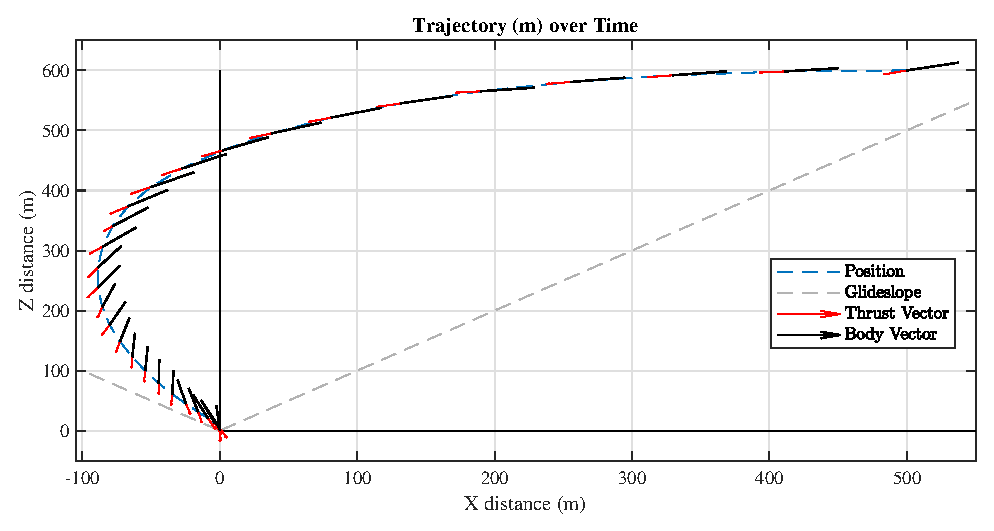
\includegraphics[width=0.75\textwidth]{figs/planar_traj.eps}
  \caption{Planar Guidance Problem: Vehicle Descends In-line with Target}
  \label{fig:planar}
 \end{figure}
% ../SCVX/code/src/controls.eps
\begin{figure}[!htbp] 
\label{planar_controls}
  \centering
  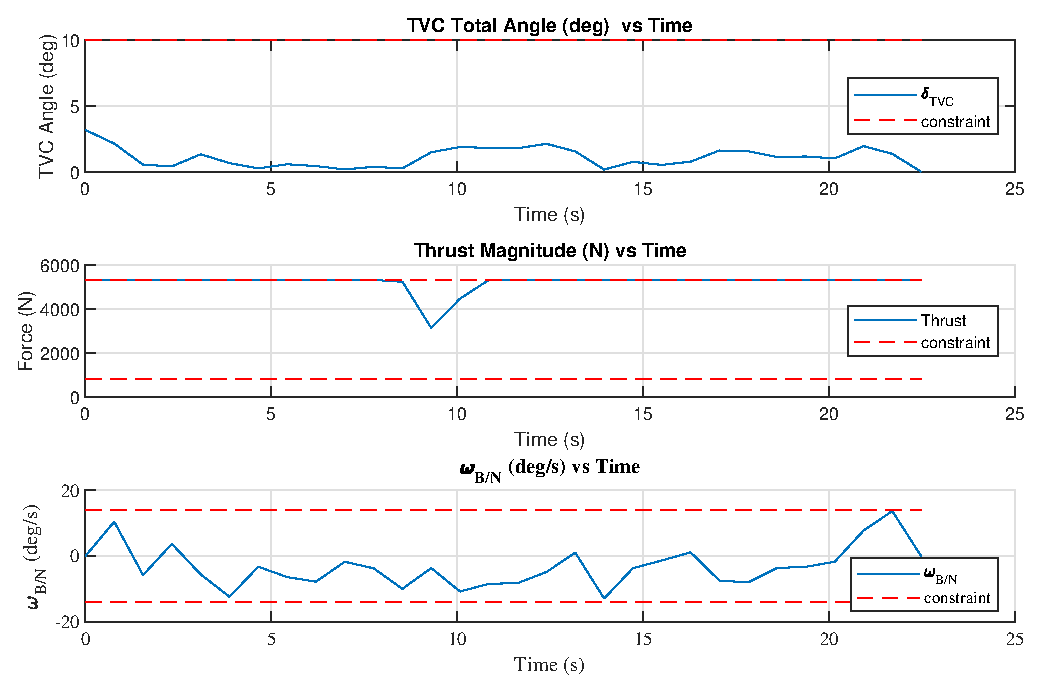
\includegraphics[width=0.65\textwidth]{figs/planar_controls.eps}
  \caption{Planar Guidance Problem: Control and Angular Rate During Landing}
  \label{fig:planarcontrols}
 \end{figure}

\begin{figure}[!htbp] 
  \centering
  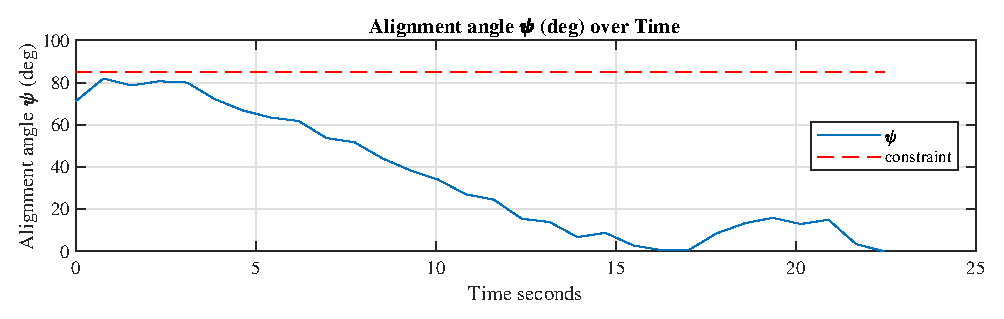
\includegraphics[width=0.7\textwidth]{figs/planar_alignment.eps}
  \caption{Planar Guidance Problem: Total Alignment}
  \label{fig:nplanar_align}
 \end{figure}


 %
The control solution in Figure \ref{fig:planarcontrols} shows how maximum thrust is used for nearly the entire duration where lateral thrust is used for attitude control while simultaneously lowering altitude control. The commanded TVC deflection angles stay within our proposed constraints. Our thrust magnitude and angular rate constraints are also met throughout the duration of the flight. For a fast pitch-over maneuvers like this, it is hard to find a trajectory where the vehicle angular rate maintains within reasonable boundaries; this scenario is restricted to below $14$ deg/s. All initial conditions and constraints are shown in Figure \ref{table:tableplanar}.


The vehicle following the planar path in Figure \ref{fig:planar} reached it's terminal state after $22.4$ seconds and with a final mass of $373.62$kg with a starting mass of $408.23$kg only using $11.7$\% of it's fuel. Additionally, the total alignment MRP constraint is shown to meet the requirement throughout the flight in Figure \ref{fig:nplanar_align}.


\section{Non-Planar Problem Solutions}
Now let us look at a non-planar problem where the initial condition of the vehicle is off-nominal and must make an out-of-plane maneuver to land on the target. The parameters and initial conditions are found in table \ref{table:tablenplanar}. Figure \ref{fig:nplanar} shows a vehicle coming towards the landing pad with an offset lateral position of 100m and with a velocity not pointed directly in-line with the target. All vehicle constraints are met. The vehicle uses maximum thrust almost the entire duration of the flight. The optimization provides a thrust-vectored solution which precisely arrests the attitude motion while meeting the translational requirements simultaneously. The simple MRP alignment constraint is met and shown in Figure \ref{fig:nplanarcontrols}.

\begin{figure}[!htbp] 
  \centering
  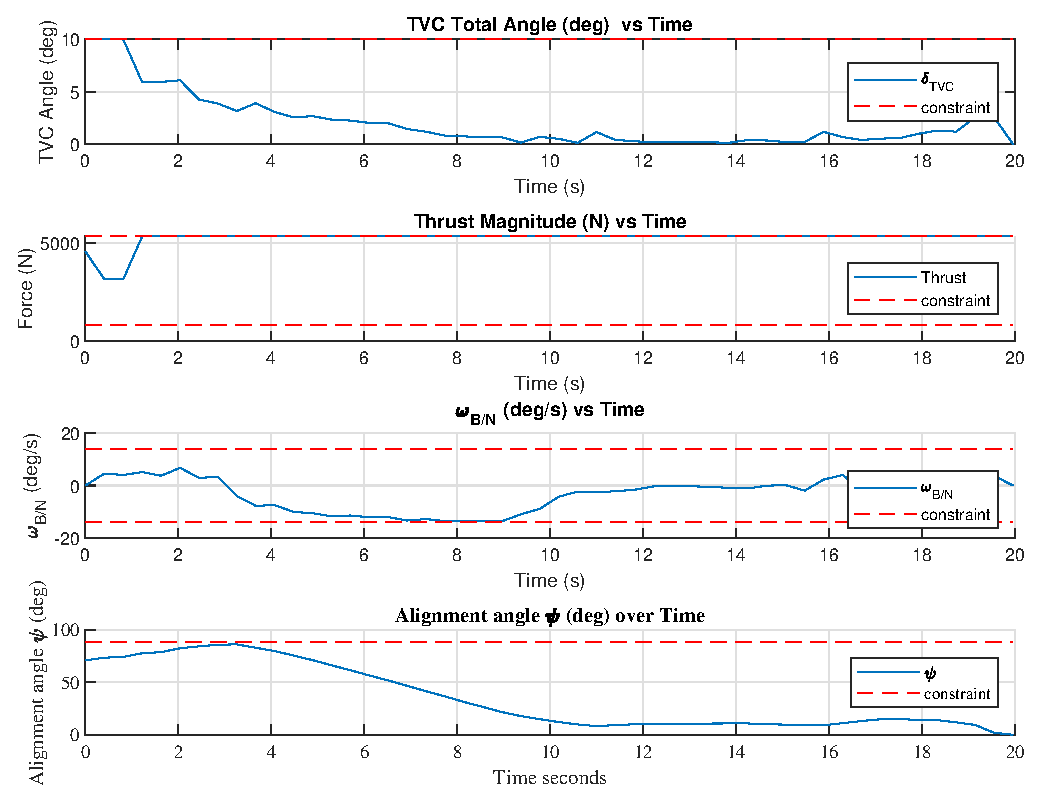
\includegraphics[width=0.65\textwidth]{figs/nonplanar_controls.eps}
  \caption{Non-Planar Guidance Problem: Controls and Angular rate of Landing Vehicle}
  \label{fig:nplanarcontrols}
 \end{figure}

\clearpage
\begin{figure}[!htbp] 
  \centering
  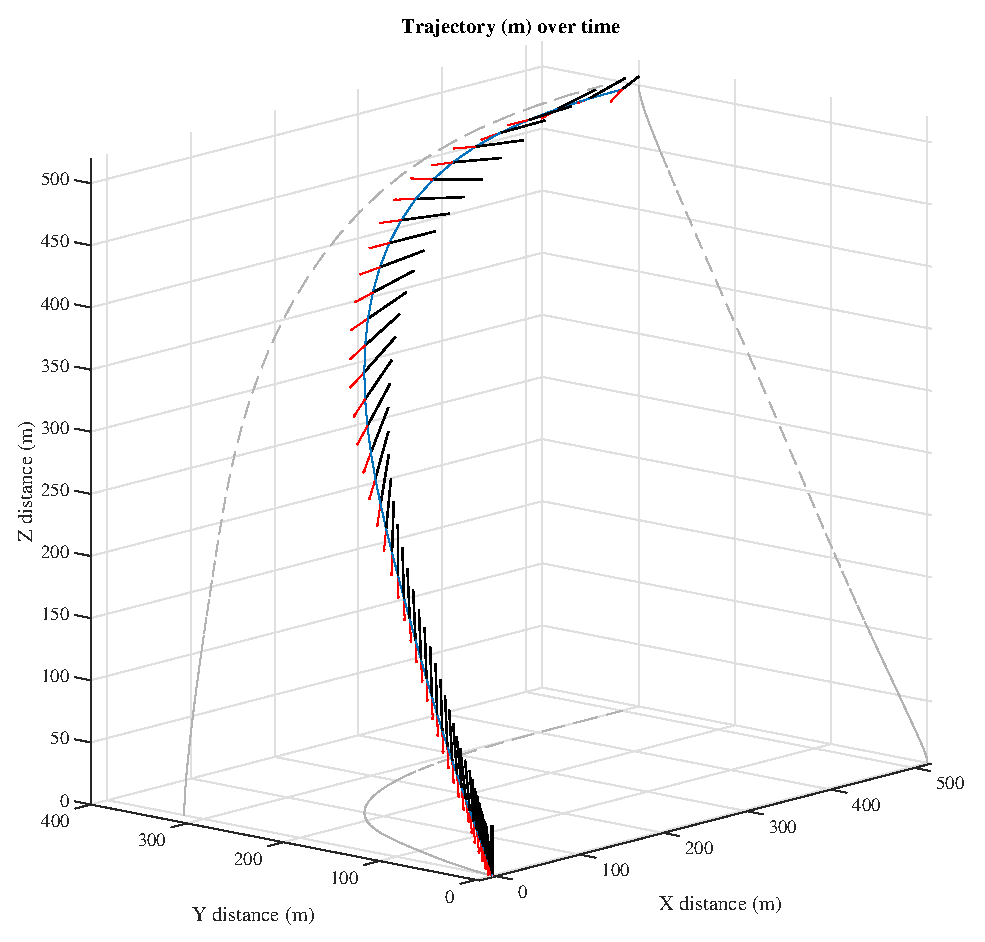
\includegraphics[width=0.8\textwidth]{figs/nonplanar_3dtraj.eps}
  \caption{Non-Planar Guidance Problem: Vehicle Approaches Offset from Target}
  \label{fig:nplanar}
 \end{figure}
 
 \begin{figure}[ht] 
  \centering
  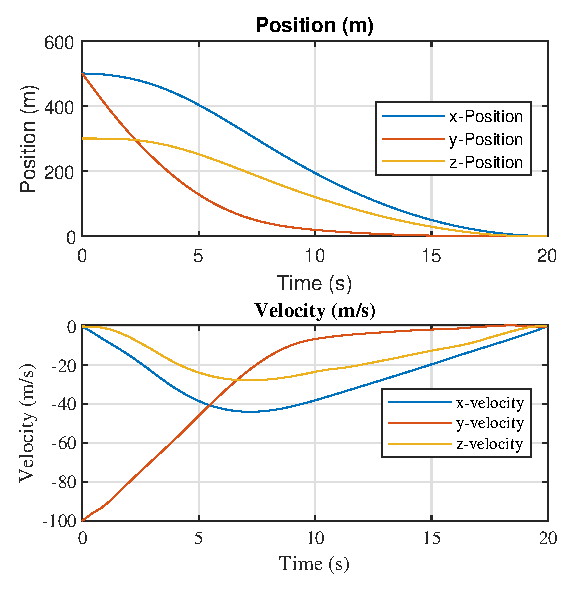
\includegraphics[width=.5\linewidth]{figs/nonplanar_rv.eps}
  \caption{Non-Planar Guidance Problem: Position and Velocity Histories}
  \label{fig:nplanar_rv}
\end{figure}

The vehicle following the non-planar path in figure \ref{fig:planar} reached its terminal state after $19.95$ seconds and with a final mass of $376.784$kg with a starting mass of $408.23$kg only using $10.6$\% of its fuel. Additionally, figure \ref{fig:nplanar_rv} shows that the terminal position and velocity constraints are met, and the vehicle reaches the landing pad with a safe terminal velocity.

\begin{table}[ht]
  \caption{Parameters Used for Non-Planar Problem}
  \centering 
  \begin{tabular}{c c c} 
    \hline\hline
    Param & Units & Value \\ [0.5ex] 
    \hline 
    $^\mathcal{N}\mathbf{g}$ 		& $U_L/U_T^2$ 	& $\hat{\mathbf{n}}_1$  \\ 
    $\alpha_{\dot{m}}$ 				& - 			& 0.0738  \\
    $m_{wet}$ 						& $U_M$ 		& 1  \\
    $m_{dry}$ 						& $U_M$ 		& 0.277  \\
    $^\mathcal{N}r_{0}$ 			& $U_L$ 		& $(0.65,0.65,0.39)$  \\
    $^\mathcal{N}v_{0}$ 			& $U_L/U_T$	 	& $(0,-0.4,0)$  \\
    $\sigma_{\mathcal{B/N}_0}$ 		& - 			& $(0,0,0.32)$  \\
    $\omega_{\mathcal{B/N}_0}$ 		& $rad/U_T$ 	& $(0,0,0)$ \\[1ex] 
    \hline
    \end{tabular}
    \begin{tabular}{c c c} 
    \hline\hline
    Param & Units & Value \\ [0.5ex] 
    \hline 
    $\gamma_{gs}$ 					& $deg$ 		& $5$  \\ 
    $\delta_{max}$	 				& $deg$ 		& $10$  \\
    $F_{max}$ 						& $U_F$ 		& $0.166$ \\
    $F_{min}$ 						& $U_F$ 		& $0.025$  \\
    $\psi_{max}$ 					& $deg$ 		& $85$  \\
    $\omega_{max}$ 					& $deg/U_T$	 	& $43.84$  \\
    $U_M$ 							& kg 			& $408.233$  \\
    $U_L$					 		& m			 	& $768.114$ \\
    $U_T$					 		& s			 	& $3.132$ \\[1ex] 
    \hline
  \end{tabular}
  \label{table:tablenplanar}
\end{table}









\clearpage
\section{Conclusion}
The successive convexification routine is a very valuable tool in that it can quickly find dynamically feasible trajectories for a wide set of vehicle constraints and parameters. It could be used as an offline tool, or a receding horizon feed-forward guidance strategy where the temporal resolution increases as the terminal state constraint gets closer. 

\section*{Acknowledgments}
The authors would like to thank Prof. Behçet Açikmeşe and the Autonomous Control Laboratory at the University of Washington.

\begin{singlespace} 
\bibliography{references}
\end{singlespace}

\end{document}
